\chapter{control Design} \label{ch:control}
%ADD intro: in this section etc
Section \ref{sec:con.nlgc} introduces nonlinear geometric control and concepts of geometric properties that are used for analysis and control design.  
%In the previous chapter, 
In the previous chapter, the configuration spaces of the system dynamics were expressed on nonlinear manifolds,.
In Section \ref{sec:con.configerr}, error functions and geometric mappings are defined on these same nonlinear manifolds in order to measure the error between current and desired states. 

In order to deal with the under-actuated nature of the system, a backstepping control approach is applied to stabilize the system .
This control design allows multiple controllers to operate in a cascaded structure, which results in the possibility to track a load position, while stabilizing the system.
The control design with its different flight modes and the corresponding controllers are discussed in Section \ref{sec:con.back}.

%controlling different states,
%which enables the control of different states, 
%resulting in the 
%stabilizing the system and tracking control
%control of the load position tracking problem.
%controllers are designed to obtain the required control inputs to stabilize the system
%are calculated by defining 


%ADD 
%deze references introduceren
%\cite{Bullo2005,Jurdjevic1997}

\newpage
\section{nonlinear geometric control}\label{sec:con.nlgc}
Many control systems are developed for the standard form of ordinary differential equations
\begin{equation}\label{key}
 \dot{x}=f(x,u) 
\end{equation}
where $ x $ is the state and $ u $ the control input. It is assumed that the state and the control input lie in Euclidean spaces, and the system equations are defined in terms of smooth functions between Euclidean spaces. However, for many mechanical systems, the configuration space can only be expressed locally as a Euclidean space. 
A nonlinear space is required to express the configuration space globally, which is discussed in the previous chapter.

geometric control Theory is the study on how geometry of the state space influences control problems. 
In control systems engineering, the underlying geometric features of a dynamic system are often not considered carefully. 
Differential geometric control techniques utilize these geometric properties for control system design and analysis.
The objective is to express both the system dynamics and control inputs on nonlinear manifolds instead of local charts. 
In contrast to locally defined linear control, nonlinear geometric control can be defined almost globally, avoiding singularities that would occur in the representation of large angles and complex maneuvering.

The design of the controllers for the \a{qr} attitude can be found in \cite{Lee2010}, and the controllers of load attitude- and position this can be found in \cite{Sreenath2013c}. Thorough stability analyses are presented in these references. For a deeper understanding of Lyapunov stability analysis in geometric control, the reader can refer to \cite{Bullo2005}.
Other control systems that are able to switch between control modes, such as the hybrid control described in \cite{Gillula2010}, require complicated reachability set analysis to guarantee safe switching between different flight modes.
%but without the use of differential geometry,  
%In contrast to such controllers, 
nonlinear geometric control does not require such analysis, as the region of attraction for each flight mode covers the configuration space almost globally. A study on global nonlinear dynamics of various classes of closed loop attitude control systems can be found in \cite{Chaturvedi2011a}. 

%
%***************************************\\
%Bart: Stability analysis goed in relatie gebracht met de scope van jouw thesis. Hier heb je wat aan en weet je wat je te wachten staat als je hybrid gaat toevoegen in further research.\\
%Nam: Het gaat eigenlijk over hybrid control zonder differential geometry. Aangepast.
%
%***************************************\\
%
%
%***************************************\\
%Bart: Bedoel je hier This is in contrast to ....
%
%Met andere woorden volgens mij klopt die zin niet helemaal toch? 
%
%En waarom haal je hier aan dat hybrid control geen complicated analysis nodig heeft? \\
%Nam: Doel is om duidelijk te maken dat die hybrid controller -zonder geometric control- júist wel complicated analysis nodig heeft, om te switchen naar andere flight modes. En de geometric controller niet. Zin veranderd: duidelijker?
%
%***************************************\\

\subsection{Error Functions}\label{sec:con.configerr}


%***************************************\\
%%ADD almost-global uitleg
%Bart: Suggestie: ALmost gloabally staat ook in de Abstract en summary. Dan lijkt het mij belangrijk. Maar wordt hier niet uitgelegd waarom almost. Waar heb je dit uitgelegd? Ik verwacht het ergens te vinden met ctrl f \\
%Nam: aan het einde van de controller uitleg. almost globally = globally minus de punten waarop het niet gestabiliseerd kan worden. Wordt gedefinieerd in domain of attraction.
%
%***************************************\\
The control of a trajectory tracking problem requires state feedback to define tracking errors, a measure of the difference between the current states and the desired states.
Since the closed-loop system dynamics evolve on nonlinear manifolds, which describe the configuration space of the \a{qr} attitude $ \in SO(3) $ and the load attitude $ \in \mathbb{S}^2 $, 
error functions are defined on these same manifolds \cite{Bullo2005}. 
These functions play a role in the definition of the potential function for the closed-loop system and form the basis for both stabilizing and tracking controllers of the \a{qr}-load system.
%Likewise, the tracking errors $ \Psi_R:SO(3)\times SO(3)\rightarrow\mathbb{R} $ and $ \Psi_q:\mathbb{S}^2\times \mathbb{S}^2\rightarrow\mathbb{R} $ are expressed on these manifolds. 
%an for the purpose of control design. 
%The derivation of the error functions can be found in \cite{Bullo2005}.
%CHECK 
%\cite{Maithripala2006}
%CHECK
%Attitude control systems naturally evolve on nonlinear configuration spaces such as $ \mathbb{S}^2 $ and $ SO(3) $. 
%Attitude tracking control is developed on $ SO(3) $, therefore it avoids singularities of Euler-Angles.
\subsubsection*{quadrotor Attitude Error}
Recall that $ R $ is the rotation matrix to describe the \a{qr} attitude, and $ R_d $ is the desired rotation matrix. To describe the relative rotation from the body frame to the desired frame, an \textit{attitude error} is defined as $ R^T_dR $. Note that $ R^T_dR $ is again a rotation matrix itself.
Based on this attitude error, the \textit{tracking error function} $ \Psi_R $ on $ SO(3) $ is chosen to be 
\begin{equation}\label{eq:psiR}
\Psi_R(R,R_d)=\frac{1}{2}tr\left[I-R_d^TR\right]
\end{equation}
such that $ \Psi_R $ is locally positive-definite about $ R^T_dR=I $ within the region where the rotation angle between $ R $ and $ R_d $ is less than $ 180^\circ $. 
It can be shown that this region where $ \Psi_R<2 $ almost covers $ SO(3) $ \cite{Lee2010c}.\\
%ADD explain
% instead of comparing all elements of rotation matrix. PsiR is a measure for the error
%ADD 
%(physical) Meaning of the error functions
%Equation  states that the variation of the rotation matrix is expressed as $ \delta R = R\hat{\eta} $ for $ \eta\in\mathbb{R}^3 $.
Using Equation \ref{eq:mod.hatvee} and \ref{eq:mod.varRq}, the derivative of the tracking error function $ \Psi_R $ with respect to R along the direction of $ \delta R=R\hat{\eta} $ for $ \eta\in\mathbb{R}^3 $ is given by
\begin{equation}\label{key}
\begin{aligned}
\mathbf{D}_R\Psi(R,R_d)\cdot R\hat{\eta}&=-\frac{1}{2}tr[R_d^TR\hat{\eta}]\\
&=\frac{1}{2}(R^T_dR-R^TR_d)^\vee\cdot\eta
\end{aligned}
\end{equation}
%By applying Equation \ref
%\texttt{\begin{equation}\label{key}
%\mathbf{D}_R\Psi(R,R_d)\cdot R\hat{\eta}=
%\end{equation}}
where the \textit{vee map} $ ^\vee:\mathfrak{so}(3)\rightarrow\mathbb{R}^3 $ is the inverse of the \textit{hat map} defined in Section \ref{sec:mod.geometric}. From this equation, the \a{qr} \textit{attitude tracking error} $ e_R \in \mathbb{R}^3$ is chosen as follows
\begin{equation}\label{eq:con.eR}
e_R=\frac{1}{2}(R_d^TR-R^TR_d)^\vee
\end{equation}
%The tracking error functions on $ TSO(3) $, the tangent space of $ SO(3) $, are defined as
%The attitude and angular velocity tracking error should be carefully chosen as they evolve on the tangent bundle of  $ SO(3) $. \cite{Lee2010c} 
It is important to note that the velocities $ \dot{R} $ and $ \dot{R}_d $ cannot be compared directly, since they do not lie in the same space. 
At time $ t=t_0 $, assume that $ R(t_0)=q$ and $R_d(t_0)=r$, then $ \dot{R} $ and $ \dot{R}_d $ lie in their own tangent spaces, denoted by $ T_qSO(3)$ and $ T_{r}SO(3)$, respectively. For this reason, $ \dot{R}_d $ must be transformed into a vector on $ T_qSO(3) $ to allow a meaningful comparison with $ \dot{R} $. 
Defining a velocity error can be achieved with a mathematical object called a \textit{transport map}, 
which enables the comparison of tangent vectors living in different spaces.\\ 
In Figure \ref{fig:con.transport}, two curves $ R(t) $ and $R_d(t)$ evolve on manifold $ SO(3) $. 
Transport map $ \mathcal{T}(q,r):T_{r}SO(3)\mapsto T_qSO(3) $ allows comparison of the velocity curves $ \dot{R} $ and $ \dot{R}_d $.
\begin{figure}[h!]
	\centering
	\makebox[\textwidth][c]{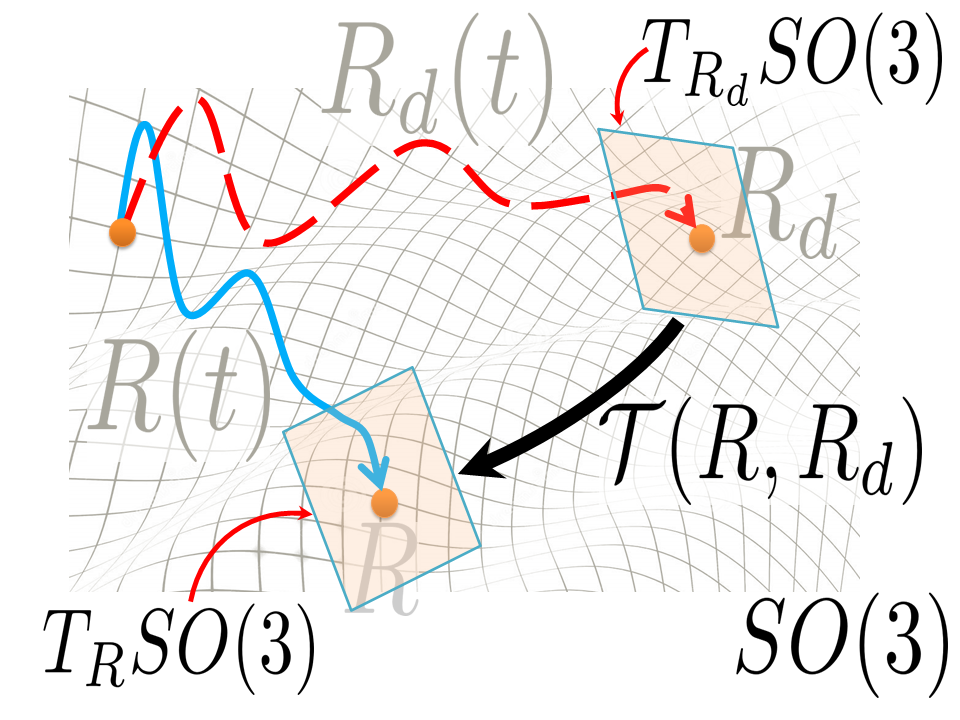
\includegraphics[width=.45\textwidth]{./StyleStuff/transport.png}}
	\caption{Transport map $ \mathcal{T}(q,r) $\label{fig:con.transport}}
\end{figure}		
%The tracking error $ \Psi_R $ and the transport map $ \mathcal{T}(q,r) $ allow the definition of error between velocity curves.

%The time derivative of the tracking error function is defined by the tracking error function $ \Psi_R $, the transport map $ \mathcal{T}(q,r)  $ and the velocity error curve $ \dot{e} $. 
% $ \dot{e} $ is a function of the transport map $ \mathcal{T}(q,r)  $. 
%Where 
The \textit{velocity error} $ \dot{e} $ is a vector field along $ R $ corresponding to the transport map.
% $ \mathcal{T}(q,r) $. 
It defines the velocity error between the curves $ R$ and $ R_d$, and is defined as
\begin{equation}\label{eq:con.dote}
\dot{e}=\dot{R}-\dot{R}_d(R_d^TR)
\end{equation}
This equation is rewritten to obtain the angular velocity tracking error, as follows
\begin{equation}\label{key}
\begin{aligned}
\dot{R}-\dot{R}_d(R_d^TR) &=R\hat{\Omega}-R_d\hat{\Omega}_d(R_d^TR) \\
&=R(\Omega)^\wedge-(RR^T)R_d\hat{\Omega}_dR_d^TR\\
&=R(\Omega)^\wedge-R(R^TR_d{\Omega}_d)^\wedge \\
&=R(\Omega-R^TR_d{\Omega}_d)^\wedge 
\end{aligned}
\end{equation}
The angular \textit{velocity tracking error} $ e_{\Omega} $ expressed in \BF  is defined as
\begin{align}\label{eq:con.eOmega}
e_\Omega&=\Omega- R^TR_d\Omega_d
\end{align}
Similar to the form of Equation \ref{eq:mod.R}, $ e_\Omega $ represents the angular velocity vector of the relative rotation matrix $ R_d^TR $, represented in \BF. Hence, it can be shown that the following equation holds
\begin{equation}\label{key}
\frac{d}{dt}(R^T_dR)=(R_d^TR)\hat{e}_\Omega
\end{equation}
%Having defined a measure 
%
%***************************************\\
%Bart: Wat is het verschil tussen de velocity error between curves R en Rd en angular velocity tracking error?\\
%Nam: velocity error $ \dot{e} $ is velocity error tussen $ \dot{R} $ en $ \dot{R}_d $.  Angular velocity error $ e_\Omega $ is de angular velocity vector van $ R_d^TR $, dus verschil tussen $ \Omega $ en $ \Omega_d $.
%
%***************************************\\

The values of the \a{qr} attitude tracking error $ e_R $ and the \a{qr} angular velocity tracking error $ e_\Omega $ 
are used later on to design control for the \a{qr} attitude.
%a controller can use this values to control

\subsubsection*{load Attitude Error}
The load attitude dynamics evolve on $ \mathbb{S}^2 $ and its tangent space $ T\mathbb{S}^2 $, where the error of the load attitude is described in a similar approach.
The error between the load attitude $ q $ and the desired load attitude $ q_d $ is defined by the error function $ q_d^Tq $. Based on the error function, the tracking error function $ \Psi_q $ on $ \mathbb{S}^2 $ is chosen to be
\begin{equation}\label{eq:psiq}
\Psi_q=1-q_d^Tq
\end{equation}
The derivative of the tracking error function $ \Psi_q $ is given by 
\begin{equation}\label{key}
d_1\Psi_q(q,q_d)=\hat{q}^2q_d
\end{equation}
From this equation, the load attitude error function $ e_q $ is defined as follows
\begin{equation}\label{eq:con.eq}
e_q=\hat{q}^2q_d
\end{equation}
Again, a \textit{transport map} is used for a comparison between the tangent vectors on different tangent spaces.
Using the tracking error $ \Psi_q $ and the transport map $ \mathcal{T}_{\mathbb{S}^2} $, a closed-loop energy function evolving on $ \mathbb{S}^2 $ is derived \cite[11.3.2]{Bullo2005}. From this energy function, the load angular velocity error function is defined as
\begin{equation}\label{eq:con.edq}
e_{\dot{q}}=\dot{q}-(q_d\times\dot{q}_d)\times q
\end{equation}
The values of the load attitude tracking error $ e_q $ and the load angular velocity tracking error $ e_{\dot{q}}$ 
are used later on to design control for the load attitude.

\subsubsection*{load Position Error}
The tracking errors for the load position and load velocity are defined as
\begin{align}\label{key}
e_x&=x-x_d\\
e_v&=v-v_d
\end{align}
where $ v_d=\dot{x}_d $. Furthermore, $ x_d(t) \in \mathbb{R}^3$ must be a smooth twice-differentiable load trajectory, such that functions are well defined. The values of the position error $ e_x$ and the velocity error $ e_v $ are used later on to design control for the load position.

\newpage
\section{Backstepping control}\label{sec:con.back}
A backstepping approach will be used in this research for the control of the load trajectory tracking problem, and is commonly used for \a{qr} control\cite{Mahony2012}. Backstepping control is a Lyapunov based control technique for the stabilization of nonlinear dynamical systems, developed by \cite{Kanellakopoulos1991}. 
The method relies on a \textit{triangular structure} of the system in a certain set of coordinates. The system is split into subsystems in a cascaded structure and recursive techniques allow a systematically design of feedback control laws and corresponding Lyapunov functions.

The control structure is created by starting with a stable system as the most inner subsystem. 
By "stepping back" from this subsystem, a control loop can be added around it containing a control law that defines a change of coordinates. 
This creates a virtual control input, that must stabilize the inner structure.
%This allows control of a new state, to guarantee the stability of the inner structure. 
The control law is designed by using states as virtual control inputs, such that each loop computes a virtual command signal for the adjacent inner loop. This is repeated until the final external control is reached.

The backstepping approach is able to calculate the control inputs $ f $ and $ M $ that are required to stabilize the \a{qr}, while several controllers are able to track different states, see Figure \ref{fig:con.loop}. 
The inner controller determines what the required control inputs are, driven by $ R_c $.  
The next controller calculates how to drive the computed rotation matrix $ R_c $ based on $ q_c $, such that the \a{qr} is stabilized.
And the last controller determines which load attitude $ q_c $ is required, such that the desired load position $ x_{L,d} $ is tracked.
\begin{figure}[h!]
	\centering
	\makebox[\textwidth][c]{\includegraphics[trim={0 0 0 12cm},clip,width=.95\textwidth]{./StyleStuff/backstepQR3.png}}
	\caption{nonlinear geometric control Loop of the QR-load system \cite{Sreenath2013c}\label{fig:con.loop}}
\end{figure}	

% EXTRA LINK
%\url{https://www.slideshare.net/ieijjournal/feedback-linearization-and-backstepping-controllers-for-coupled-tanks}
%\url{http://www.control.lth.se/media/Education/EngineeringProgram/FRTN05/2013/lec09_2013eight.pdf}
%We want to design a state feedback u=u(x) that stabilizes
%\begin{equation}\label{key}
%\begin{aligned}
%\dot{x}_1&=f(x_1)+g(x_1)x_2\\
%\dot{x}_2&=u
%\end{aligned}
%\end{equation}
%Idea is to see system as a cascade connection. Design controller first for inner loop, then for the outer.
%
%Back-Stepping Lemma
%\textbf{Lemma}: Let $ z=\begin{pmatrix}x_1,\cdots,x_{k-1}\end{pmatrix}^T$ and 
%\begin{equation}\label{key}
%\begin{aligned}
%\dot{z}&=f(z)+g(z)x_k\\
%\dot{x}_k&=u
%\end{aligned}
%\end{equation}
%Assume $ \phi(0)=0 $, $ f(0)=0 $,
%\begin{equation}\label{key}
%\dot{z}=f(z)+g(z)\phi(z)
%\end{equation}
%stable, and $ V(z) $ a Lyapunov function (with $ \dot{V}\leq-W $). Then, 
%\begin{equation}\label{key}
%u=\frac{d\phi}{dz}\begin{pmatrix}
%f(z)+g(z)x_k
%\end{pmatrix}-\frac{dV}{dz}g(z)-(x_k-\phi(z))
%\end{equation}
%stabilizes $ x=0 $ with $ V(z)+(x_k-\phi(z))^2/2 $ begin a Lyapunov function.
%
%The backstepping approach determines how to stabilize the {\displaystyle \mathbf {x} } \mathbf {x}  subsystem using {\displaystyle z_{1}} z_{1}, and then proceeds with determining how to make the next state {\displaystyle z_{2}} z_{2} drive {\displaystyle z_{1}} z_{1} to the control required to stabilize {\displaystyle \mathbf {x} } \mathbf {x} . Hence, the process "steps backward" from {\displaystyle \mathbf {x} } \mathbf {x}  out of the strict-feedback form system until the ultimate control {\displaystyle u} u is designed.
%***************************************\\

Since the \a{qr} has only four actuators, it is not possible to control all \a{DOF}s of the \a{qr}-load system simultaneously. The backstepping approach allows control of different flight modes in which a combination of \a{DOF}s is controlled. The flight modes and their functions are defined below in order, from the most inner loop to the most outer loop.
\begin{outline}
	\1 QR Attitude controlled Mode 
	\2 Track a desired QR attitude $ R_d(t) $ or commanded signal $ R_c(t) $
	\2Optional tracking of a desired heading direction $ b_{1_d}(t) $, the first column of $ R_d(t) $
	\2 Calculate the control input $ M $ for the \a{qr}-load system
	\1 load Attitude controlled Mode 
	\2 Track a desired load attitude $ q_d(t) $ or commanded signal $ q_c(t) $
	\2 Calculate a computed \a{qr} attitude $ R_c $ for the \a{qr} attitude controller
	\2 Calculate the control input $ f $ for the \a{qr}-load system	
	\1 load Position controlled Mode
	\2 Track a desired load position $ x_{L,d}(t) $
	\2 Calculate a computed load attitude $ q_c $ for the load attitude controller
	\2 Calculate the control input $ f $ for the \a{qr}-load system		
\end{outline}
where the subscript $d $ denotes a desired tracking reference, which must be given whenever it is not calculated by a controller. For example in Figure \ref{fig:con.qrattalone}, where the \a{qr} attitude controller works as a standalone controller, without taking load attitude and position into account.
The subscript $ c $ denotes a computed tracking reference, calculated by the controllers. 
\begin{figure}[h!]
	\centering
	\makebox[\textwidth][c]{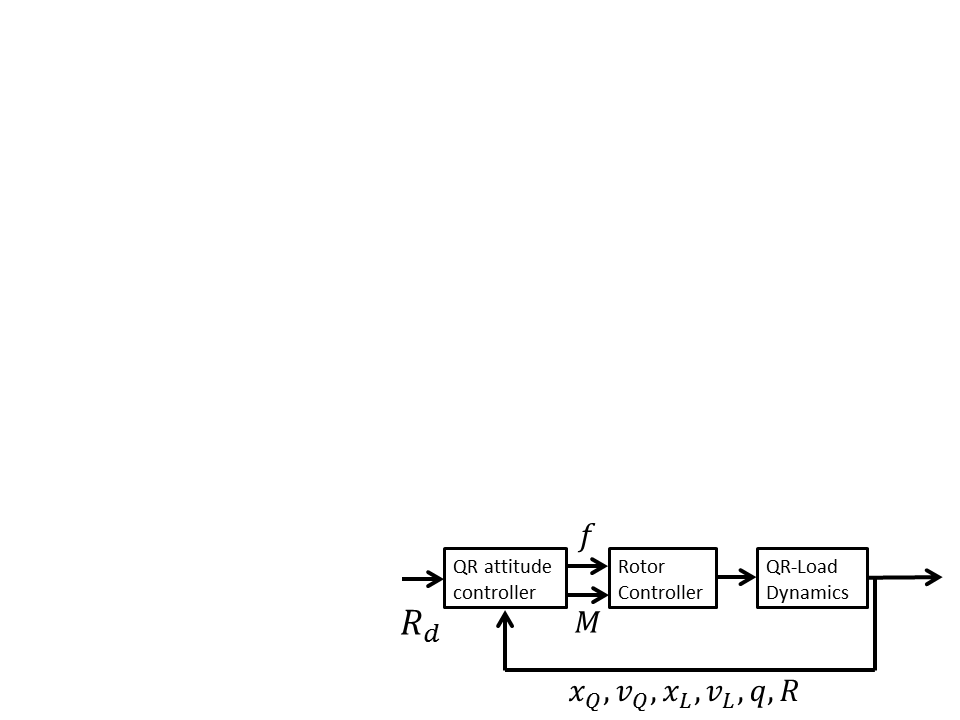
\includegraphics[trim={10cm 0 0 13.5cm},clip,width=.6\textwidth]{./StyleStuff/qrattalone.png}}
	\caption{QR Attitude controller\label{fig:con.qrattalone}}
\end{figure}		


%CHECK NODIG??
%More detailed derivations of the equations in the following sections can be found in Section \ref{sec:}.

%value that is calculated as a . The difference in this notation is whether the signal is a predefined desired signal, or a signal computed by a controller.
%The controller that is used in this research is shown in Figure \ref{fig:con.loop}. The lowest levels have the highest bandwidth and are in control of the rotor rotational speeds $ \omega_i $, the total force $ f $ and moments $ M $. The next level controls the load attitude $ q $, and the top level controls the load position $ x_L $. 

\subsection{quadrotor Attitude Tracking}\label{sec:con.qratt}
The \a{qr} Attitude controlled Mode is designed to control the \a{qr} attitude by tracking a smooth desired \a{qr} attitude $ R_d(t) $.  
Analysis of the error dynamics $ e_R $ and $ e_\Omega $ requires the calculation of their time derivatives.\\
Using Equations \ref{eq:con.eR} and \ref{eq:con.eOmega}, the derivative of the attitude tracking error $ e_R $ can be written as
\begin{equation}\label{key}
\dot{e}_R=\frac{1}{2}(R_d^TR\hat{e}_\Omega+\hat{e}_\Omega R^TR_d)^\vee
\end{equation}
The derivative of the angular velocity tracking error $ e_\Omega $, follows from Equations \ref{eq:mod.R}, \ref{eq:con.eOmega} and $ \hat{\Omega}_d\Omega_d =0$, such that
\begin{equation}\label{eq:con.deOmega}
\dot{e}_\Omega=\dot{\Omega}+\hat{\Omega}R^TR_d\Omega_d-R^TR_d\dot{\Omega}_d
%\dot{e}_\Omega=J^{-1}(-\Omega\times J\Omega + M)+\hat{\Omega}R^TR_d\Omega_d-R^TR_d\dot{\Omega}_d
\end{equation}
Recall from Equation \ref{eq:mod.R}, that the kinematics equation for the desired attitude can be written as
\begin{equation}\label{eq:con.dotRd}
\dot{R}_d=R_d\hat{\Omega}_d \text{ and } \hat{\Omega}_d=R_d^T\dot{R}_d
\end{equation}
%From this follows that 
The desired angular acceleration $ \dot{\Omega}_d $ follows from the following equation
\begin{equation}
\begin{aligned}
\dot{\hat{\Omega}}_d&=(\dot{R}_d^T\dot{R}_d)+(R_d^T\ddot{R}_d)\\
&=(R_d\hat{\Omega}_d)^T(R_d\hat{\Omega}_d)+(R_d^T\ddot{R}_d)\\
&=-\hat{\Omega}_d\hat{\Omega}_d+R_d^T\ddot{R}_d
\end{aligned}
\end{equation}
such that,
\begin{equation}\label{eq:con.dOmegad}
\dot{\Omega}_d=(-\hat{\Omega}_d\hat{\Omega}_d+R_d^T\ddot{R}_d)^\vee 
\end{equation}
By substituting Equation \ref{eq:mod.qratt} into Equation \ref{eq:con.deOmega}, the following equation is obtained
\begin{equation}\label{eq:con.dOmega}
\dot{e}_\Omega=J^{-1}(-\Omega\times J\Omega + M)+\hat{\Omega}R^TR_d\Omega_d-R^TR_d\dot{\Omega}_d
\end{equation}
From this, the control input $ M $ is defined \cite{Lee2010c}, and consists of a proportional term, a derivative term and a canceling term, as follows
\begin{equation}\label{eq:con.M}
M = -k_Re_R-k_\Omega e_\Omega+\Omega\times J\Omega-J(\hat{\Omega}R^TR_d\Omega_d-R^TR_d\dot{\Omega}_d)
\end{equation}
Rapid exponential convergence of the attitude error function and angular velocity error function can be achieved by adding
the parameter \lsymb{$ \epsilon $}{Tuning parameter to enable rapid exponential convergence of $ e_R, e_\Omega $} to
Equation \ref{eq:con.M}  as done in \cite{Sreenath2013c}, where $ 0<\epsilon<1 $,, given by
\begin{equation}\label{eq:con.Meps}
M = -\frac{1}{\epsilon^2}k_Re_R-\frac{1}{\epsilon}k_\Omega e_\Omega+\Omega\times J\Omega-J(\hat{\Omega}R^TR_d\Omega_d-R^TR_d\dot{\Omega}_d)
\end{equation}
Substituting Equation \ref{eq:con.Meps} into Equation \ref{eq:con.dOmega} results in the time derivative of the angular velocity tracking error, given by
\begin{equation}\label{eq:con.JdeOmega}
\dot{e}_\Omega=J^{-1}(-\frac{1}{\epsilon^2}k_Re_R-\frac{1}{\epsilon}k_\Omega e_\Omega)
\end{equation} 
for any positive constants $ k_R, k_\Omega $.\\
% and where \lsymb{$ \epsilon $}{Tuning parameter to enable rapid exponential convergence of $ e_R, e_\Omega $} is the parameter to enable rapid exponential convergence of the attitude- and angular velocity error functions, such that $ 0<\epsilon<1 $ \cite{Sreenath2013c}
%such that Equation \ref{eq:con.deOmega} is reduced to
%\begin{equation}\label{eq:con.JdeOmega}
%J\dot{e}_\Omega=-k_Re_R-k_\Omega e_\Omega
%\end{equation}
%for any positive constants $ k_R, k_\Omega $.\\
Equation \ref{eq:mod.hattrace} is used to rewrite the time derivative of $ e_R $ as follows
 %rewrite the attitude velocity error $ \dot{e}_R $ as follows
 \begin{equation}\label{eq:con.deR}
 \begin{aligned}
 \dot{e}_R&=\frac{1}{2}(R_d^TR\hat{e}_\Omega+\hat{e}_\Omega R^TR_d)^\vee\\
 &=\frac{1}{2}(tr[R^TR_d]I-R^TR_d)e_\Omega \equiv C(R_d^TR)e_\Omega 
 \end{aligned}
 \end{equation}
where $ \parallel C(R_d^TR)\parallel_2\leq 1 $, such that $ \parallel\dot{e}_R\parallel\leq\parallel e_\Omega \parallel  $ for all $ R^T_dR\in SO(3) $, guaranteeing that $ \dot{e}_R $ will be bounded, whenever $ e_\Omega $ is bounded. 
%Equations \ref{eq:con.JdeOmega} and \ref{eq:con.deR} are used in a stability analysis of the controller, 
In \cite{Lee2010} it is proven that the Lyapunov functions, which are functions of the error dynamics $ e_R,e_{\Omega},\dot{e}_R,\dot{e}_{\Omega}$ described above, are non-increasing and bounded. With this controller stability analysis, it is proven that the zero equilibrium of the closed loop tracking error $ (e_R,e_\Omega)=(0,0) $ is exponentially stable, if the initial conditions satisfy
\begin{equation}\label{eq:dom1}
\Psi_R(R(0),R_d(0))<2
\end{equation}
\begin{equation}\label{eq:dom2}
\parallel e_\Omega(0)\parallel^2<\frac{2}{\lambda_M(J)}\frac{k_R}{\epsilon^2}(2-\Psi_R(R(0),R_d(0)))
\end{equation}
where \lsymb{$ \lambda_M(\cdot) $}{Maximum eigenvalue} denotes the maximum eigenvalue. \\
Furthermore, there exist constants $ \alpha_R,\beta_R>0 $ such that
\begin{equation}\label{eq:con.proofPsiR}
\Psi_R(R(t),R_d(t)) \leq min\left\lbrace 2,\alpha_Re^{-\beta_Rt}\right\rbrace 
\end{equation}
%T is defined by Equations . 
Equations \ref{eq:dom1} and \ref{eq:dom2} determine the domain of attraction, which is the region in which the trajectory of the system is able to converge to an asymptotically stable equilibrium point. 
The domain of attraction almost covers $ SO(3) $, this is referred to as almost-global exponential attractiveness.

Note that the tracking of the \a{qr} attitude does not require any specification of the thrust magnitude $ f $. During this flight mode, the translational motion can only be controlled partially, which makes this flight mode suitable for attitude maneuvers with short time periods. For a \a{qr} system without load, in \cite{Lee2010} a tracking controller is described that calculates both a thrust magnitude $ f $ and total moment $ M $ in order to track a \a{qr} position trajectory.

\subsection{Load Attitude Tracking}\label{sec:con.loadatt}
%ADD Dependent of what values? 	How to choose parameters.
The load Attitude controlled Mode is designed to track a desired load attitude $ q_d $.
In order to influence the load dynamics, see Equation \ref{eq:mod.loadatt}, the load attitude controller calculates a computed \a{qr} attitude $ R_c $ for the \a{qr} attitude controller, which replaces $ R_d $.\\
The commanded directions of the body frame axes are defined by $ R_c $, and is defined as follows
\begin{equation}\label{eq:con.R}
R_c = \begin{bmatrix}
b_{1c}; b_{3c}\times b_{1c};b_{3c}
\end{bmatrix}
\end{equation}
$ \Omega_d $ is replaced by $ \Omega_c $, where $ \Omega_c $ is defined by
\begin{equation}\label{key}
\hat{\Omega}_c=R_c^T\dot{R}_c
\end{equation}
which will influence the \a{qr} attitude dynamics, see Equation \ref{eq:mod.qratt}.\\
The unit vector $ b_{1c} $ is the first column of $ R_c $ and is constructed by normalizing the projection of a desired heading angle $ b_{1d}\in \mathbb{S}^2 $ onto the plane normal to $ b_{3c} $, see Figure \ref{fig:con.b1c}. Defining $ b_{1c}\in\mathbb{S}^2$ orthogonal to  $ b_{3c}$ guarantees that $ R_c \in SO(3) $ \cite{Lee2010c}.
\begin{figure}[h!]
	\centering
	\makebox[\textwidth][c]{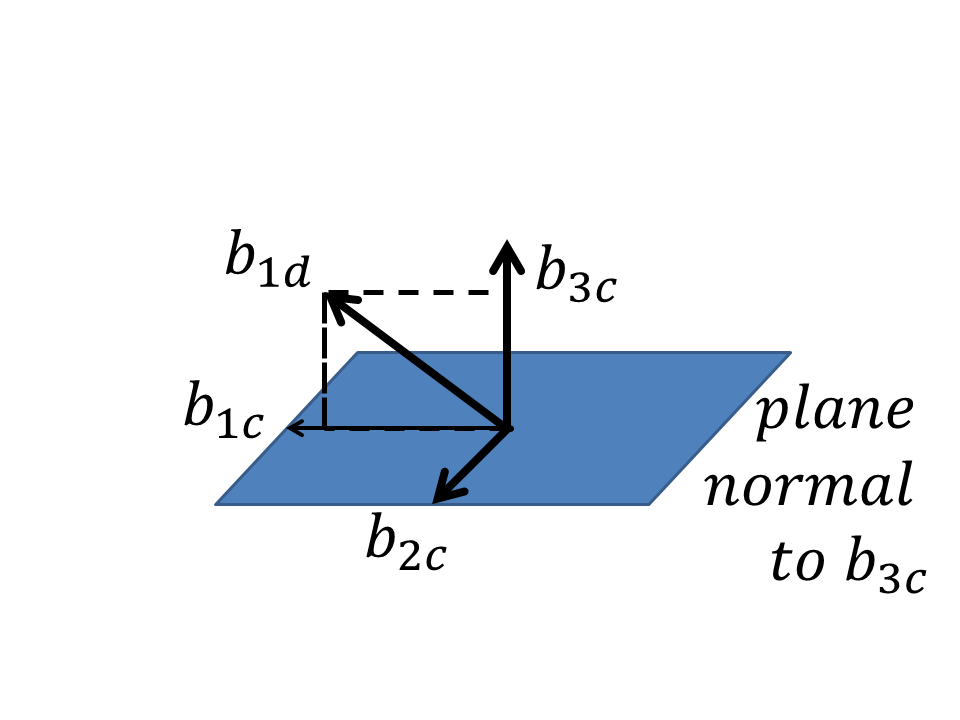
\includegraphics[trim={0 3cm 0 6cm},clip,width=.45\textwidth]{./StyleStuff/b1c.png}}
	\caption{Construction of  $ b_{1c} $ to define $ R_c $\label{fig:con.b1c}}
\end{figure}	

 $ b_{1c} $ is defined as follows
\begin{equation}\label{key}
b_{1c}=-\frac{1}{||b_{3c}\times b_{1d}||}(b_{3c}\times(b_{3c}\times b_{1d}))
\end{equation}
Such that $ b_{2c}= b_{3c}\times b_{1c}$, and $ b_{1d} $ is chosen, not parallel to $ b_{3c} \in \mathbb{S}^2 $, the third column of $ R_c $.\\
 $ b_{3c} $ is defined by a normalization of $ F $,
\begin{equation}\label{eq:con.b3c}
b_{3c}=\frac{F}{||F||}
\end{equation}
where $F $ is defined by a normal component $ F_n $, a proportional-derivative component $ F_{pd} $ and feedforward control force $ F_{ff}$
\begin{equation}\label{eq:con.F}
F=F_n-F_{pd}-F_{ff}
\end{equation}
% control forces for a system  are derived . 
The inclusion of $ F_n $ ensures that $ b_{3c} $ is always well defined. $ F_n $ is defined as
\begin{equation}\label{eq:con.Fn}
F_n=-(q_d\cdot q)q
\end{equation}
The control forces $ F_{pd} $ and $ F_{ff} $ are defined for trajectory tracking in \cite[11.2.5]{Bullo2005} as follows
\begin{equation}\label{eq:con.Fpd}
\begin{aligned}
F_{pd}&=-k_P\hat{q}^2q_d-k_D(\dot{q}-(q_d\times\dot{q}_d)\times q)\\
&=-k_qe_q-k_\omega e_{\dot{q}}
\end{aligned}
\end{equation}
and
\begin{equation}\label{key}
F_{ff}=m_QL\langle\!\langle q,q_d\times\dot{q}_d\rangle\!\rangle_{\mathbb{R}^3}(q\times \dot{q})+m_QL(q_d\times \ddot{q}_d)\times q
\end{equation}
for positive constants $ k_q, k_\omega $.\\	
This controller affects the control input $ f $, which is defined as
\begin{equation}\label{eq:con.floadatt}
f=F\cdot Re_3
\end{equation}
and the control input $ M $ will be defined as
\begin{equation}\label{eq:con.Mloadatt}
M = -\frac{1}{\epsilon^2}k_Re_R-\frac{1}{\epsilon}k_\Omega e_\Omega+\Omega\times J\Omega-J(\hat{\Omega}R^TR_c\Omega_c-R^TR_c\dot{\Omega}_c)
\end{equation} 

It is proven in \cite{Sreenath2013c} and \cite[Lemma 11.23]{Bullo2005} that the zero equilibrium of the closed loop tracking error $ (e_q,e_{\dot{q}},e_R,e_\Omega)=(0,0,0,0) $ is exponentially stable, if the initial conditions satisfy
\begin{equation}\label{eq:dom3}
\Psi_q(q(0),q_d(0))<2
\end{equation}
\begin{equation}\label{eq:dom4}
\parallel e_{\dot{q}}(0)\parallel^2<\frac{2}{m_QL}{k_R}(2-\Psi_q(q(0),q_d(0)))
\end{equation}

The domain of attraction is defined by Equations \ref{eq:dom1}, \ref{eq:dom2}, \ref{eq:dom3} and \ref{eq:dom4}. Equation \ref{eq:dom3} states that the initial load attitude error should be less than $ 180^\circ $, which means that the controller achieves almost-global exponential convergence for load attitude $ q $.
Furthermore, there exist constants $ \alpha_q,\beta_q>0 $ such that
\begin{equation}\label{eq:con.proofPsiq}
\Psi_q(q(t),q_d(t)) \leq min\left\lbrace 2,\alpha_qe^{-\beta_qt}\right\rbrace 
\end{equation}

\subsection{Load Position Tracking}\label{sec:con.loadpos}
The load Position controlled Mode is designed to track a desired load position $ x_{L,d} $. 
Analysis of the error dynamics $ e_x $ and $ e_v $ requires the calculation of their time derivatives.\\
The derivative of the load position error $ e_x $ is given by
\begin{equation}\label{eq:con.dex}
\dot{e}_x = e_v
\end{equation}
and from Equation \ref{eq:mod.loadpos} and given that $ \dot{e}_v=\ddot{x}_L-\ddot{x}_{L,d} $ follows
\begin{equation}\label{eq:con.dev}
(m_Q+m_L)\dot{e}_v=-(m_Q+m_L)(ge_3+\ddot{x}_{L,d})-m_QL(\dot{q}\cdot\dot{q})q+(q\cdot fRe_3)q
\end{equation}
Equations \ref{eq:con.dex} and \ref{eq:con.dex} are used in a stability analysis of the controller. 
The load position controller calculates a computed load attitude $ q_c$ for the load attitude controller. $ R_d $ and $ q_d $ are replaced by $ R_c $ and $ q_c $, respectively. 
In order to stabilize the error dynamics, it is proven in \cite{Sreenath2013c} that the required computed load attitude is defined as
\begin{equation}\label{eq:con.q}
q_c = - \frac{A}{||A||}
\end{equation}
where
\begin{equation}\label{eq:con.A}
A = -k_xe_x-k_ve_v+(m_Q+m_L)(\ddot{x}_{L,d}+ge_3)+m_QL(\dot{q}\cdot\dot{q})q
\end{equation}
%with $ e_x=x_L-x_{L,d} $ and $ e_v=\dot{x}_L-\dot{x}_{L,d} $.
Furthermore, Equation \ref{eq:con.Fn} is redefined as
\begin{equation}\label{key}
F_n=(A\cdot q)q
\end{equation}
which is substituted in Equation \ref{eq:con.F}, resulting in a new control input $ f $. 

This controller ensures that the zero equilibrium of the closed loop tracking error $ (e_x,e_v,e_q,e_{\dot{q}},e_R,e_\Omega)=(0,0,0,0,0,0) $ is exponentially attractive, if the initial conditions satisfy
\begin{equation}\label{eq:dom5}
\Psi_q(q(0),q_c(0))<\psi_1<1
\end{equation}
\begin{equation}
\parallel e_{x}(0)\parallel^2<e_{x_{max}}
\end{equation}
where $ e_{x_{max}} $ and $ \psi_1 $ are fixed design depended constants. 

The domain of attraction is defined by Equations \ref{eq:dom1}, \ref{eq:dom2}, \ref{eq:dom5} and the following equation
\begin{equation}
\parallel e_{\dot{q}}(0)\parallel^2<\frac{2}{m_QL}{k_q}(\psi_1-\Psi_q(q(0),q_d(0)))
\end{equation}

%\section{Stability Analysis}\label{sec:con.sta}
%
%Normally Lyapunov Analysis is 
%
%
%Lyapunov Analysis on SO3 x R3 and S2 x R3
%
%
%
%%In addition, the LaSalle invariance result and related Lyapunov results apply to closed-loop vector fields defined on these manifolds. 
%
%However, since the manifolds $ SO(3) $ and $ \mathbb{S}^2 $ are compact, the radial unboundedness assumption cannot be satisfied; consequently, global asymptotic stability cannot follow from a Lyapunov analysis on Euclidean spaces [40], and therefore must be analyzed in alternative ways [19]–[23].\cite[p.43]{Chaturvedi2011}
%
%[40]:
%[19]:
%[20]:
%[21]:
%[22]:
%[23]:
%
%
%\cite{Chaturvedi2011} summarizes global results on attitude control and stabilization for a rigid body using continuous time- invariant feedback. The analysis uses methods of geometric mechanics based on the geometry of the special orthogonal group $ SO(3) $ and the two-sphere $ \mathbb{S}^2 $.
%
%%ADD 
%%Justify choice of parameters. Up to what level can we push the system? Where can we find more info about domain of attractions.
%%How to choose parameters and how to select gains for errors


\section*{Summary}
In this chapter, control design based on nonlinear geometric control is discussed.
%It is pointed out that 
%The main difference 
What is particular in this control technique, is the fact that error functions are defined on non-Euclidean manifolds, similar to the manifolds that describe the configuration space of the system.
Since these manifolds are locally Euclidean, local stability properties of a closed-loop equilibrium solution can be determined by using standard Lyapunov methods. 
Based on these error functions, controllers are designed in a backstepping approach, enabling both load position tracking and stabilization of the system.
Using the geometric properties of the system allows the design of globally defined controllers that ensure almost-global convergence of the \a{qr} attitude and load attitude.
In order to test the control performance of a load position tracking objective, experiments are defined in the next chapter. 

% CHECK Chaturvadi?
%Stability analysis is different from a Lyapunov analysis on Euclidean spaces.







